\documentclass{article}
\usepackage[utf8]{inputenc}
\usepackage[letterpaper, margin=1in]{geometry}
\usepackage{amsmath}
\usepackage{setspace}
\usepackage[authordate,backend=biber,natbib]{biblatex-chicago}
\usepackage{graphicx}
\usepackage{csquotes}
\usepackage{hyperref}
\usepackage{booktabs}
\usepackage{wrapfig}
\hypersetup{
    colorlinks=true,
    linkcolor=blue,
    citecolor=blue,
    filecolor=magenta,      
    urlcolor=blue,
}

\addbibresource{pesch.bib}

\title{Heinrich Pesch and the Anglo-German Divide in Economics}
\author{William R. Hauk, Jr.\thanks{The author thanks participants at the Southern Economics Association and the Catholic Research Economists Discussion Organization online seminar, and particularly Jes\'{u}s Fern\'{a}ndez-Villaverde, Arnd K\"{u}ppers, Claudio Lucarelli, and two anonymous referees for helpful comments.  All remaining errors are the author's.  Phone:  +1-803-777-6044  Email:  hauk@moore.sc.edu.}\\University of South Carolina}
\date{May 2021}

\begin{document}
\maketitle

\doublespacing
\begin{abstract}
The Rev. Heinrich Pesch, S.J. was a German economist and social philosopher who was an active scholar from the 1890s to 1920s.  His work had a significant impact on a generation of German Catholic social thinkers and particularly the papal encyclical \emph{Quadragesimo Anno}.  His method of social analysis, which he called Solidarism, was informed by Catholic Social Thought, but based on natural law principles that he argued were accessible to all people of good will.  This article argues that, although his school of thought did not survive the Nazi and World War II years, many of his ideas had a lingering effect on Economic thought for the German center-right.  This influence may be contrasted with the center-right in Britain, where there was a strong divorce between Christian social thinking and Economics.  Consequently, a gap emerged between Economic policy in Germany and Britain, which contributes to tensions over economic policy that remain today.

\textbf{Keywords:}  Heinrich Pesch, Catholic Social Thought, Solidarism

\textbf{JEL Codes:}  B15, B31, F02, Z12

\end{abstract}

\section{Introduction}

The Rev. Heinrich Pesch, S.J. was a German economist and social philosopher who was active as a scholar between the 1890s and 1920s.  While he is relatively little known in the English-speaking world today, his views influenced a generation of German Catholic social thinkers, culminating in Pope Pius XI’s encyclical \emph{Quadragesimo Anno}, which was published five years after his death.  The social philosophy that he espoused, called Solidarism, proceeded from his study of Economics and the relatively nascent field of modern Catholic Social Thought.  In it, he attempted to derive a method of social analysis that would avoid the two major competing ideologies of his day, individualist liberalism, and Marxist socialism.  Against these currents of thought, he proposed the bonds of social solidarity combined with subsidiarity as a means of combating modern ills.\medskip

As this essay will show, although the system of Solidarism did not survive the Nazi era and World War II in Germany, it had a continuing impact on the economic thinking of the center-right in Germany.  This difference is in sharp contrast to the influence of Anglican economic thought (or, ultimately, a lack thereof) on the British center-right.  As will be demonstrated below, there was a relatively early separation of economic and theology amongst Anglicans, which caused the British right to evolve in a more laissez-faire direction, influenced by the relative secularism of modern neoclassical economics.  In contrast, the work of Catholic social thinkers like Pesch helped to create a strain of economic thinking on the German right that was closely tied to theology.  We can see this influence in the types of economic institutions set up in Germany in the post-war era, such as the workers’ councils and the social market system.  Even as German society has gone through a marked secularisation in recent decades, these institutions have remained.  As a result, Pesch’s economic thought has an enduring effect in Germany and through this channel, the economic policies of the European Union.\medskip

This essay will start by looking at Pesch’s biography and the major characteristics of his philosophy of Solidarism.  It will then describe how that system creates a view of the market and the economy that is frequently at odds with modern neoclassical economics as understood in the U.K. (and by extension, America).  Finally, it will look at the developments in the influence of Christian social thought in center-right economic thought in the United Kingdom and Germany and speculate on what this separation means for the current economic tensions between the U.K. and continental Europe.

\section{Pesch's Biography and Economic System}

\subsection{Biography}

\begin{figure}
    \centering
    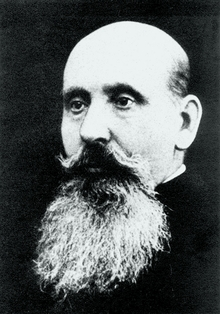
\includegraphics{Heinrich_Pesch.jpg}
    \caption{Rev. Heinrich Pesch, S.J.;
        By Unknown author - \href{http://www.unitas-ruhrania.org/index.php?section=news&amp;cmd=details&amp;newsid=1170}{Unitas Ruhrania}; Public Domain, \href{https://commons.wikimedia.org/w/index.php?curid=25140631}{Wikimedia Commons}
    }
    \label{fig:peschphoto}
\end{figure}

The Rev. Heinrich Pesch, S.J. was born in 1854 in Cologne in what was then the Rhine Province of the Kingdom of Prussia.  After studying law at the University of Bonn, where he first became acquainted with economic theory, he joined the Society of Jesus in 1876.  Because of the anti-Catholic policies of Bismarck’s \emph{Kulturkampf}, he spent his novitiate with the Jesuits in the Netherlands and then studied for four years in Lancashire England.  It was there that he observed firsthand the effects of the British Industrial Revolution, but even more so, the effects of its liberal economic order on the working classes.  It was this experience which motivated him to study social issues, especially related to the question of labor.\citep{schuyler1953}\medskip

He completed his theological studies shortly before Pope Leo XIII ushered in the modern era of Catholic Social Teaching with his encyclical \emph{Rerum Novarum} in 1891.  Inspired by the encyclical, Pesch began a period of informal study of economic thought.  Eventually, he enrolled at the University of Berlin, where he pursued higher studies in Economics under the faculty there.  He then devoted the rest of his life to writing on social and economic subjects while working at the Jesuit House of Writers in Luxembourg, ``where he was delighted to have at his disposal all of the important economic literature from England, America, France, Austria, Switzerland and Germany." \citep[p. 3]{mulcahy1952}\medskip

While his writings are voluminous, three works in particular stand out as being of lasting importance and are available in English translation.\footnote{Perhaps one of the greatest factors limiting Pesch’s exposure to the broader world of Economics was, until recently, the lack of English translations of his works.  The late Rupert Ederer, Professor of Economics at the State University College at Buffalo, spent several years of his retirement translating Pesch’s works into English.  All direct citations of Pesch in this essay are due to Ederer’s translations.}  The first, focusing on the tension between the great social philosophies of his day, was \emph{Liberalismus, Socialismus, und Christliche Gesellschaftsordnung (Liberalism, Socialism, and Christian Social Order)} published in 1900.  The second focused more on a specific ethic for Economic policy and was entitled \emph{Ethik und Volkswirtschaft (Ethics and the National Economy, 1918)}.  Finally, his great work, which he spent about 23 years composing and filled 10 volumes, was the \emph{Lehrbuch Der National\"{o}konomie (Teaching Guide to Economics)} published between 1905 and 1923.  This last work outlined an economic system that attempted to incorporate the social philosophy of the medieval scholastic philosophers – particularly Aquinas – into a scientific study of Economics.\medskip

Pesch’s health began to fail after the publication of the last volume of the \emph{Lehrbuch}, and he passed away in 1926.  However, his greatest triumphs may have come posthumously.  Two of Pesch’s students, the German Jesuits Rev. Gustav Gundlach, S.J. and Rev. Oswald von Nell-Breuning, S.J., were instrumental in the drafting of Pope Pius XI’s encyclical \emph{Quadragesimo Anno} issued in 1931 for the 40th anniversary of \emph{Rerum Novarum}.  The encyclical, while not explicitly using the term ``solidarity" introduced the Peschian principles of subsidiarity, occupational groups, and social justice and charity to Catholic Social Teaching. \citep{ederer1991}  While not specifically citing Pesch, the word ``solidarity" appears frequently in many subsequent papal encyclicals, particularly Pope Paul VI’s \emph{Populorum Progresso} and Pope John Paul II’s \emph{Laborem Exercens}.\footnote{It would, of course, be wrong to claim that Pesch invented the idea of solidarity, given its use as a principle in a variety of contexts, both religious and secular.  However, it is clear that, after his work, the term makes a more prominent appearance in Catholic Social Thought.}

\subsection{Solidarism}

Two aspects of Pesch’s work stand out in making him essential to understanding the difference between German and British economic thought.  The first is that he developed his economic philosophy partially in response his first-hand experience of British industrialization and classical liberalism.  The second is that, while Pesch, as a Jesuit priest, was motivated by Catholic Social Teaching, as a citizen of a territory with a Protestant (and occasionally actively anti-Catholic) government, he needed to argue in a way that would be compelling to non-Catholics as well.\medskip

Pesch wrote at a time when mainstream economics in the English-speaking world was undergoing its neoclassical revolution.  Because of the triumph of this approach in contemporary economics, it is perhaps difficult for economists trained in modern English-speaking programs to think of the economy in the same way that Pesch did.  Rev. Richard Mulcahy, S.J., writing in the 1940s and 50s, directly contrasted Pesch’s view of the economy with that of the British economic thinker Lionel Robbins. \citep{mulcahy1949}  Robbins famously claimed that ``economics is entirely neutral between ends; that, in so far as the achievement of any end is dependent on scarce means, it is germane to the preoccupations of the economist." \citep[p.23]{robbins1932}  By contrast, Pesch, influenced by the social philosophy of Aristotle and Aquinas, took a fundamentally teleological approach to economics.  That is, he saw economics as a practical, rather than purely speculative, science.  Economics was a science concerned with the best means of obtaining a goal, rather than an exercise in working out the conclusions of a set of premises (such as the behavior of a rational utility maximizer).\medskip

Furthermore, the existence of a goal for the economy gives us a normative criterion for choosing between the different ends that an economic decision-maker might face.  Economics could not be neutral to the ends that people choose, but it can only favor those ends that serve the ultimate goal of the economy.  For Pesch, this central goal of the economy was to provide for the material welfare of society.  \citep{mulcahy1949}  In Pesch’s words, a good economy consisted of, ``A sound stratification of property ownership with moderate wealth, a broad middle class, and the assurance of a dignified human level of living for even the humblest classes – that is what the material well-being of a nation calls for, and what all must therefore cooperate to bring about." \citep[p. 180]{pesch1998}\footnote{Pesch's emphasis on a broad distribution of property ownership echoes some of the arguments made by the English Distributists, Hilaire Belloc and G.K. Chesterton, who were also inspired by \emph{Rerum Novarum}.  A clear difference between the two schools of thought is in Pesch's attempt to build broader institutions that ended up being compatible with the German Social Market system described below.  For an essay on the relationship between Pesch and the Distributists, see \citet{storck2008}.}  While preference satisfaction (as is assumed by most utilitarian neoclassical theories) certainly plays a role in this end, the goal exists outside of individual preferences.\medskip

Pesch therefore sought to develop a system of economic thought that would avoid two extremes identified in Pope Leo XIII’s encyclical \emph{Rerum Novarum} – that of economic liberalism and socialism.  According to Catholic Social Thought, liberalism was in error because it posited a society made up of atomized individuals who interacted with each other solely on a contractual basis when necessary to satisfy mutual interests.  Socialism made the opposite error by seeing individuals solely as parts of the broader society, or as members of different classes of that society. \citep{schuyler1953}  On the other hand, Catholic Social Thought sees man as an intrinsically social being, being created in the image of God, with a vocation to love. \citep[no. 34]{pcjp2004}  While a man has a vocation as an individual, he can only attain that vocation in relationship with others.  While it is perhaps useful to think of Pesch’s thought as a \emph{via media} between liberal individualism and socialist collectivism, it should be noted that this is more of an Aristotelian golden mean incorporating the insights of both rather than a lazy compromise between the two. \citep{koslowski2000}\medskip

Pesch named his economic system ``Solidarism."  He saw it as a logical extension of Catholic Social Teaching.  However, he used philosophical principles derived from natural law, thus believing that his system should be accessible to all people of good will.  Solidarism was built around the twin principles of solidarity and subsidiarity from Catholic Social Thought.  Solidarity in Pesch’s thought existed at four distinct levels.  First, solidarity should exist among all people by virtue of their common Creator.  Second, solidarity should exist among members of a family.  Third, solidarity should exist among citizens of the same state.  Finally, solidarity should exist among members of a common vocational group (including management, employees, and different firms within an industry). \citep[pp. 69-70]{pesch1998}\medskip

By making solidarity a function of several different levels of society, Pesch sought to balance the tension existing between the two principles of solidarity, by which we express concern for society’s common good, and subsidiarity, by which we express concern for the freedom of individuals and intermediary institutions in society.  Social solidarity is thus an imperative in Pesch’s system, but the multiple levels of solidarity put limits on the ability of higher-level institutions to usurp the activities proper to lower-level institutions.  While this form may take on different concrete realizations in different circumstances, according to Pesch, ``What is essential to it, however, is the concept of organic community:  community and along with communal responsibility, the principle of moral organism." \citep[p. 81]{pesch1998}  As part of a ``moral organism" the members of a community necessarily exist in relation to each other, but also possess their own status as moral subjects with their own vocations and ends that society is bound to respect and nurture.\medskip

Economic liberalism, by contrast, adopts a position of methodological individualism, where subjective preference satisfaction (usually represented by a utility function) is the primary metric of the economy’s performance.  Thus, the market determined price, which is typically believed to allocate scarce resources in a means that maximizes that utility, becomes the primary criterion by which the efficiency of the market is evaluated.  This methodological choice leads to an implicitly utilitarian normative criterion, even if, as noted below, many economists in this tradition wish to separate positive and normative concerns.\medskip

Pesch’s teleological approach, by contrast, says that the efficiency of an economic arrangement can only be evaluated in reference to the ends that the economy is supposed to serve.  It differs from the neoclassical approach on two dimensions.  First, the end of the economy is objective, rather than subjective.
\begin{displayquote}
Each individual and the community, along with those in authority, have to comport themselves in such a way, and establish economic conditions in such a manner, or enable them to be structured in such a way, that the ultimate goal of life in the political order and society – the genuine welfare of all and the free development of the personalities along with all of the wealth of their particular talents and capacities – can achieve their full realization for every member of society according to the full extent that this is possible.\footnote{\citet[p.60]{pesch1998}}
\end{displayquote}
Second, that end is inherently social.  In Pesch’s words “In order to achieve many essential and legitimate objectives in our lives we cannot dispense with continual human assistance.  For us, there is no such thing as absolute self-sufficiency.” \citep[p. 7]{pesch1998}  Therefore, an economics that looks at welfare in a purely individualistic sense is likely to go astray.\medskip

This idea is particularly apparent in Pesch’s treatment of just price theory.  Pesch focuses considerably on the idea that a freely agreed upon market price may not necessarily be just.  While the theory permeates Pesch’s writings, it is certainly not original to Pesch.  Indeed, the similar views can be traced back to as far as Aristotle in the \emph{Nicomachean Ethics}.  While nearly all ethicists would agree that an economic transaction involving physical coercion would be immoral, Aristotle and the medieval scholastics who referred to him added the idea of economic coercion. \citep{langholm2014}  Economic coercion may exist when economic power – defined in Langholm as ``the power to dispose of something that others need"  – between two sides of an exchange is imbalanced.  When the party to an exchange who has a greater amount of economic power exercises that power to alter the terms of that exchange in their favor, economic coercion is exercised, and the terms of the exchange may be considered unjust.\medskip

It is essential in a system that stresses the teleological nature of the economy that justice prevail in economic transactions.  It cannot be good for the national welfare if someone acts unjustly, regardless of the immediate material gain.  In the case of economic transactions, commutative justice requires that the value of the goods exchanged be equivalent on both sides of the transaction.  Of course, a person will normally only exchange in a transaction if she expects to have some positive gain by the by engaging in the transaction.  In neoclassical terms, a person will buy a good if the marginal utility of the good for her is greater than the marginal utility of money that she uses to purchase a good.  Thus, Pesch makes a distinction between the ‘use value’ of the good being exchanged – which is the subjective valuation of the good for the individuals engaged in the transaction – and the ‘exchange value’ – which is ``the general estimation… appraised in terms of the wants of the entire community." \citep[p. 215]{pesch1998}  That is, while individuals will have their own subjective valuations of a good based on their own circumstances, the general wants of the community are what gives a good its value in economic transactions.  The divergence between these two values are what makes economic exchange possible.  A good may have little value to me due to lack of necessity or an over-abundance, but it may have a greater value to a large number of other people in society.\medskip

Exchange value will, of course, vary in different times and places and is not necessarily a precise amount, but rather a general estimation.  What is necessary for commutative justice is that the price reflect this general estimation – i.e. that buyers and sellers exchange the good at a just price.  Of course, this price will fluctuate in response to the normal operations of supply and demand and should be sufficient to cover the legitimate costs of production.  In many circumstances, a competitive market price will accurately reflect the exchange value of a good.  However, two scenarios are highlighted by Pesch wherein the market price could diverge from a just price.\footnote{This list is meant to be exemplary rather than exhaustive.}  The first is when ``powerful forces and interests simply dominate the market in a one-sided manner." \citep[p. 221]{pesch1998}  To use the terms of modern economics, this situation occurs when one side of the transaction has considerably more market power than the other, such as in monopoly or monopsony, and a buyer or seller may not be able to freely choose to take place in a transaction.  The other is when one side of the transaction lacks sufficient information and is therefore unable to make an informed estimation of a good’s value.\footnote{Interestingly, Pesch seems to be anticipating here some of the insights of information economics for which later economists George Akerlof, Michael Spence, and Joseph Stiglitz would be awarded the Nobel Prize in Economics in 2001.}\medskip

Given Pesch’s emphasis on society as a moral organism, I would add one more factor elaborated in more recent economic theory to the determination of the just price – that of economic externalities.  Certain types of economic activity, whether embodied in production or consumption, can generate harms or benefits for members of society who are not party an economic exchange.  The most used example in current economic texts is environmental pollution.  When I drive a gasoline-consuming car, I do not (in the absence of other taxation or regulation) directly pay for the pollution generated by my activity, and thereby inflict costs on other members of society that is not reflected in the price of my gasoline consumption.  This activity violates the principle of equivalence – the cost that I pay does not reflect the sacrifices made by other people – thereby making the market price of gasoline unjust.\footnote{Another recent writer, John Mueller, notes that another factor missing from Pesch's creation of a ``neo-scholastic" economics is Augustine's theory of gifts, which receives more attention from the original scholastics than it does in Pesch.  In a society that is a moral organism, gratuitous transfers would be important. \citep[pp. 117-125]{mueller2010}}\medskip

This view contrasts with the classical liberal view that the absence of physical coercion (in which case, a party to a transaction can always walk away from a deal) presumptively makes a transaction mutually beneficial and, therefore, just.  Indeed, Langholm notes that the later scholastics, such as the School of Salamanca, dropped the idea of economic coercion from Catholic discourse.  In that school’s view, nearly all economic transactions are made under binding constraints, and therefore, less than ideal circumstances.  Therefore, insofar as we think voluntary transactions can be mutually beneficial, and even voluntary transactions are made with varying degrees of economic necessity, it follows that transactions made even under economic necessity can be mutually beneficial.\medskip

However, this observation does not rule out a role for economic coercion.  Walking away from a deal may be technically possible for both parties, but it may not be equally so for both.  A person who needs to sell her labor-power in exchange for wages to survive may refuse to work for a particular employer, but in the absence of other potential employers, refusal may not be a realistic choice, giving that employer greater bargaining power.  Similarly, the outcome of a transaction may be efficient in the sense that it is Pareto-improving, but a wide variety of distributional outcomes can be Pareto-improving.  Economic coercion may therefore exist and be an important factor, even in the absence of physical coercion.\medskip

Echoes of the economic coercion model are reflected in Pesch’s views of the just price.  Indeed, in a rather blistering criticism of Pesch from a classical liberal perspective, Abram Harris claims that ``For all the ethical verbiage in which his ideas concerning wages are couched, what Pesch really gives is a ‘force’ theory of wages, which, incidentally, is to a great extent exemplified in present practices of trade-unions.  If the impersonal determination of rewards by the market is generally superseded by ‘bargaining power’ as Pesch seems to propose, the determination of wages and other income shares would degenerate into a contest of organized grab." \citep[pp. 46-47]{harris1946}  It seems unlikely that Pesch would substantially disagree with the first part of the claim – the point of collective bargaining is, after all, to give workers more power in wage negotiations.  However, he would probably take issue with the second part of the statement.  In particular, he might question if wage determination is as ``impersonal" as Harris claims in an unregulated market, or even if such an outcome would be desirable.\medskip

Because wages provide the primary form of sustenance for most workers, those workers do not have an outside option with respect to whether they want to work, and their ability to seek work in different industries or locations may be highly constrained.  Conversely, at least on the margin, many employers may easily be able to substitute between different workers, different production locations, or different production technologies.  As such, in a market that is imperfectly competitive, an employer may have more bargaining power, which would keep wages lower than in an equilibrium where bargaining power is more equally distributed.  Institutions such as collective bargaining and government regulation of wages and working conditions could potentially counteract this bargaining power and restore a more efficient equilibrium.  Pesch would also probably note that ``efficiency" in the neoclassical sense is not the only criterion by which an economic outcome should be evaluated – he would rather state that it should be evaluated by the extent to which it allows for a society to secure the material welfare of its people.  It is noteworthy, however, that the approach of Pesch anticipated some of the insights of modern neoclassical economics in terms of equilibrium outcomes.\medskip

Pesch was echoing to a large degree the arguments found in \emph{Rerum Novarum} \citep[no. 49]{leoxii1891}, which would then be elaborated on at greater length in \emph{Quadragesimo Anno} \citep[no. 29-30]{piusxi1931}.  Pope Pius XI noted that in the years since his predecessor’s encyclical ``They [liberal governments] were with criminal injustice denying the natural right to form associations to those who needed it most to defend themselves from ill treatment at the hands of the powerful."  Thus, workers (and perhaps workers and employers) associations were to be defended on two grounds.  The first is through the natural right to association, which would justify their existence regardless of the economic consequences.  Secondly, they also are necessary to protect workers from more powerful actors.  Wage determination is thus most justly set not solely through an impersonal market, but rather through the creation of institutions where workers band together to offset power imbalances.  Justice here comes, not through impersonal interactions between individuals, but a recognition of differences in the bargaining power of different groups.\medskip

An interesting application of the theory of the just price in Pesch’s writings is his perspective on usury.  The medieval Church and its scholars did not permit the taking of interest on a loan, but the modern Church, in practice, does not seem to object to moderate rates of interest.  Pesch saw this phenomenon, not as a change in Church doctrine, but rather as a legitimate development due to changes in economic circumstances.  His contention was that, in the medieval era, the relative lack of economic growth and investment in capital meant that the was no real opportunity cost to lending for those who had a surplus of money, and thus no justification for a return to them for doing so.  However, the development of a modern economy meant that there was a general opportunity to make gains through the investment of funds, and therefore, lending money now represented a real sacrifice on the part of those with excess funds.\footnote{For a further discussion on Pesch’s theory of interest and usury, see the appendix to chapter 5 in \citet{mulcahy1952}.}  Similarly, we can say that changes in opportunities for exchange due to an opening of trade may legitimately change the exchange values of goods, and thus, their just prices.  This perspective is different from economists who posit a ‘time-value’ of money or ‘reward for abstinence’ that justifies the taking of interest on a loan.  Pesch argued that there is no intrinsic time-value to money, but rather that the general opportunity to make gains through investment over time is what gives money such a time-value.\medskip

From the discussion above, one might be tempted to conclude that Pesch was fundamentally hostile to economic thought generally.  On the contrary, he claims that ``Both sciences [Economics and Ethics] have a lot to learn from each other.  However, that is not the same as saying that Economics can cut itself off from the moral law, or even abstract from it." \citep[chap. 10]{pesch2004}  Furthermore, moral theology is not sufficient by itself to create an economic system:  ``Religion cannot produce grain; it cannot do away with physical ills."\footnote{Quoted in \citet[p. 151]{mueller1951}.}  Economics, as an autonomous science, contributes a lot to our understanding of the conditions for material prosperity.  But, as one educated in the Thomistic tradition, Pesch argued that truth could not contradict truth.  Something could not be simultaneously economically correct and ethically incorrect.  Hence, Economics can make a contribution to human reason by helping us to better understand the implications of policies and actions affecting material well-being, but it cannot at the same time divorce itself from ethical imperatives.\medskip

In summary, Pesch’s theory of Solidarism treated economics in a manner different from neoclassical theory.  Most relevantly for this essay are four big differences.  First, economics is a practical science in that it serves a definite end – that of providing for the material welfare of society.  Second, because economics serves that end, the performance of an economy cannot be measured solely using the satisfaction of subjective utility functions.  The economy must be evaluated in terms of that end.  Relatedly, a market-determined price is not always just.  It is just to the extent that it satisfies the demands of commutative justice and serves the ends of the economy.  Finally, because that end is communal, solidarity between different groups in society is essential to satisfying that end.  An economy cannot be simply an impersonal system of atomized individuals.  As we will see below, this difference in view set forth by Pesch would have implications that lasted into the future.

\section{Roots of the Anglo-German Divide}

\begin{figure}
    \centering
    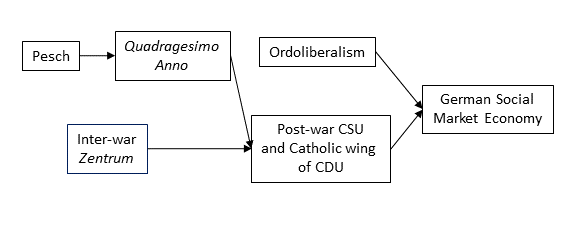
\includegraphics{Figure1.png}
    \caption{Causal Mechanism Outlined in this Article}
    \label{fig:causalmechanism}
\end{figure}

Pesch would die in 1926, and the war years and the post-war era were not exceedingly kind to the project of forming a distinctly Catholic approach to economics that avoided both liberal capitalism and Marxist socialism.  In particular, the idea of Solidarism as a stand-alone economic system became discredited due its similarities with Corporatism, which in turn was harmed by its association with the defeated fascist regimes.  Furthermore, the decline of Thomism as the leading philosophical current in Catholic thought in the years leading up to the Second Vatican Council weakened some of the intellectual foundations of the project of building a distinctly Catholic social system.  Finally, the increasing level of secularization of European life in the post-war era did not provide a fertile ground for explicit appeals to Catholic principles in the organization of society.\citep{almodovarteixeira2008}\medskip

However, it would be a mistake to assume that none of the Pesch-era principles survived the war.  In particular, the German postwar ``economic miracle" that resulted in the German Social Market economy merits attention.  Partisan cleavages in Germany during both the interwar and postwar period would ensure that Catholic Social Thought would find a niche in postwar Germany.  In an essay on religion and the formation of modern political parties in Western Europe, Thomas Ertman notes that, in many Western European countries, religious divisions have a large amount of explanatory power, perhaps even more than class cleavages.\citep{ertman2009western}  Specifically, he notes that several countries developed ``parties of religious defense" designed to protect the rights of the Catholic Church.  In interwar Germany, this party was the Catholic \emph{Zentrum}, which contended both against both Protestant conservatives and an anti-clerical left to develop a distinctive Catholic approach to politics.  While this party would eventually be subsumed by the rise of the Nazis, it helped to form both the first postwar German Chancellor, Konrad Adenauer, and the Bavarian Christian Social Union (CSU).\medskip

In contrast, Ertman notes that such a party did not arise in the United Kingdom (or, to pick a predominantly Catholic nation, France) where the Tories already formed a party devoted to protecting the ancient privileges of both the aristocracy and the established church.  While the preservation of religious institutions was a partial motivator of that party, religion itself was not a major division in British politics after the settlement following the Glorious Revolution.\medskip

The fact that Pesch’s theories, especially on just wages and prices, had a significant impact on Catholic Social Teaching (CST) gave them an opening to influence public policy on the European continent.  While left-wing parties naturally gravitated towards structural theories of economic outcomes, frequently of Marxist inspiration, many post-war European Christian Democratic parties of the center-right found inspiration in CST, which influenced the development of the so-called ``social market" economies of the post-war world.  More is said about the German example below.\medskip

In contrast, in the English-speaking world, CST historically had less influence, especially among center-right parties, who tended to look upon Catholics (and especially Catholic politicians) with a certain level of nativist suspicion.  In the case of England itself, the officially established church was the Church of England.  Anglican social thought did have an influence over public policy for a time.  Most directly, Anglican bishops sat ex-officio in the House of Lords.  Many of the great 19th century English reformers, such as Wilberforce, Shaftesbury, and Gladstone, were very explicitly motivated by Christian charity. \citep{hawtrey2014}\medskip

However, as noted by \citet{emmett2014}, even in the 19th century, a ``separation" developed between economics and theology in the British universities, creating what he called a Non-Overlapping Magisteria (NOMA).  By the end of the 19th century, Cambridge Professor John Neville Keynes formally divided economics between a ``positive science" and a ``normative art." \citep{keynes1904}  This distinction was developed further in the English-speaking world by \citet{robbins1932} and \citet{friedman1953}.\medskip

A strong distinction between positive and normative analysis in Economics need not necessarily lead to a neglect of normative analysis.  However, it is evident that, in practice, the increasing autonomy of Economics, and the desire to guard it as a ``positive science" has tended to discourage economists from speaking on normative matters as economists.\medskip

As noted above, a key distinction between Pesch and the neoclassical economists was to make this distinction between Economics as a practical, as opposed to speculative, science.  If economics is to be a practical science – that is a science geared towards generating a particular good – then there must be a clear notion of the good to which Economics must aim.  In Pesch’s case, this good was defined by the social teachings of the Catholic Church (though again he believed that the principles contained therein could be accessible to all people of good will).  Economics was a tool with which to pursue to the common good of society and needed to aim towards that end.  As such, Economics was not a fully autonomous science, but rather was closely tied to Ethics and Politics.\medskip

In contrast, in the neoclassical view, Economics was a completely autonomous discipline.  In the words of Robbins, ``Economics is entirely neutral between ends…  Economics is not concerned with ends as such." \citep[p. 24]{robbins1932}  Milton Friedman, writing a couple decades after Robbins, argued that a positive vs. normative distinction was necessary to the progress of Economics.  ``Currently in the Western world, and \emph{especially in the United States}, differences about economic policy among disinterested citizens derive predominantly from different predictions about the economic consequences of taking action – differences that in principle can be eliminated by the progress of positive economics – rather than from fundamental differences in basic values.” [emphasis added] \citep[p. 5]{friedman1953}\medskip

To say that Economics is neutral or not concerned with ends does not, of course, mean that Economics cannot be adapted to, say, the ends of Solidarism or other social philosophies.  However, by explicitly removing the discussion of ends from Economics, an emphasis on the strict autonomy of Economics as a positive science may discreetly alter the ends of economists themselves, who, by not explicitly reflecting on the ultimate ends of their actions, tend to confuse the proximate ends most commonly studied by economics (surplus maximization, gross domestic product, etc.) with the ultimate ends which the economy might serve (human well-being, societal flourishing, etc.)  Indeed, Frank Graham argued – even in 1942 – that the technical complexity of modern economics requires a degree of specialization of knowledge that mastery of technique was emphasized to the detriment of reflection on the ends sought by that technique. \citep[p. 29]{graham1999}\footnote{Citation from \citet{yuengert2004}}  As noted above, neoclassical economics, by stressing utility maximization as a welfare criterion, often implicitly sneaks in utilitarianism as a social doctrine without reflecting on that choice.\medskip

A science of Economics that is purely positive, does not reflect on ultimate ends, and is speculative in nature presents a sharp contrast with the understanding of Economics outlined by Pesch – a science that is inherently normative as well as positive due to its direct dependency on Ethics.  This emphasis on a higher order that Economics must respect tends to lead to a greater emphasis on regulation of the market.  Reviewing Pesch’s work, Stephen Krason paraphrases him by stating, ``Self-interest and self-love are always present, and indeed, they have a rightful role in economic life; they can also be destructive forces, however. So, the solidarist seeks to regulate them—as he would regulate freedom, in general (the existence of which makes man uniquely dignified)—in accordance with the higher standard of justice and in a way that respects both the individual and the community." \citep{krason2009}  Thus, we see a break between the neoclassical school, which was initially (though certainly not ultimately) associated with Anglo-American economists, which exalted the working of an autonomous market, and the Solidarist approach championed by Pesch.  (See also \citet{mulcahy1951} and \citet{yenni1951}.) \medskip

These differing ideas about the relationship between Economics, Politics, and Ethics had important implications for the way that center-right economic policy developed in the English-speaking world vs. Germany in the post-war world.  The Catholic-inspired Solidarist school had a big impact on subsequent German economic policy, while the Neoclassical school developed largely in the absence of any influence from the religious establishment in England.

\section{German Postwar Miracle}

The economic policy pursued by Konrad Adenauer and Ludwig Erhard during the postwar era in West Germany has typically been described by the term ``ordoliberalism" and was built on a particular reading of the interwar German economic crisis.  As noted by \citet[p. 351]{hien2013}, “For the ordoliberals, the crisis of Weimar was the result of the capturing of the state by economic and political interests.  The ruling coalition of Social Democrats and Catholics, with their strong auxiliary organizations and trade unions, had built an association state (\emph{Verb\"{a}ndestaat}) that had overburdened and entangled the state in welfare commitments.”  Therefore, the solution was to unburden the state of these commitments and to promote free economic competition.  In this respect, the ordoliberal view was not much different from the classical liberal view, with the notable exception that the ordoliberals wanted a state powerful enough to overcome these associational groupings.\medskip

However, the governing Christian Democratic Union (CDU) consisted of a coalition of Protestants and Catholics, reflecting the view of Adenauer (a veteran of the interwar Catholic \emph{Zentrum}) that narrow sectarian parties were not up to the task of defending democracy against the far right and far left.  While Protestants (e.g. Erhard) tended towards the ordoliberal view, Catholics in the CDU were still very much under the influence of the corporatism of \emph{Quadragesimo Anno}, and thereby, of Pesch.\medskip

There has been debate over whether or not ordoliberalism and Catholic solidarism were very much in tension with each other.  Taking a position on one end of the spectrum is Ralf Dahrendorf, who claimed in a lecture on the German Social Market economy that ``Anyone who talks about the social market economy in Germany ... means Ordoliberalism plus Catholic social teaching, two incompatibilities. But theoretically incompatible things do not have to be absurd in practice. We live with contradictions all the time and even profit from them. It is one of Konrad Adenauer's historical merits that he endured the contradiction between market economy and social policy, and even made it a program."\footnote{I am indebted to Arnd K\"{u}ppers for translating key phrases from Dahrendorf's lecture from the original German.} \citep{dahrendorf2004} \medskip

Conversely, \citet{kuppers2015} argues that the differences between the two schools of thought have been exaggerated.  On the contrary, he argues that they are both complementary.  K\"{u}ppers notes that Protestant ordoliberals such as Wilhelm R\"{o}pke and Walter Eucken in particular contributed a strong concern for social justice embedded within a market framework.  Most of the ordoliberals were active members of the the political resistance against Hitler, and many of the religiously-oriented ones were members of the Lutheran ``Confessing Church" that stood against the ``German Christian" movement that gave support to the Nazis.\medskip

Whether Ordoliberalism and Solidarism were fundamentally incompatible or not, the two schools formed the postwar German center-right.  The ordoliberal Erhard faction tended to dominate the immediate postwar years.  As noted by \citet{hien2013}, the biggest economic reform of the late 1940s was the ending of price controls put in place during the war years.  This reform was strongly ordoliberal in character, opposed by Catholics in the CDU, and given credit for a short boom in the West German economy.  However, the increased demand for industrial goods and rearmament in West Germany after the onset of the Korean War gave the Catholic faction leverage to push for a more corporatist system.  The rest of Adenauer’s term in office would represent a back and forth between the corporatists and ordoliberals.  The corporatists won on industrial relations, works councils, and generous pension system, the ordoliberals won on strong antitrust rules and a central bank famously committed to price stability.  This tug-of-war created the German Social Market Economy.  While the social market might have fallen short of the distinctive system thoroughly infused with Catholic Social Thought envisioned by Pesch, the ``Rhine Capitalism" model was very much influenced by him and his legacy among German Catholics.

\section{Brexit and Conclusion}

These contrasting histories are of no mere academic interest.  These divergent views of the relationship between Christianity and the economy arguably contribute to some of the tension between Germany and the U.K..  Center-right parties dominated post-war governments in both countries.  As of June 2019, the Conservative Party in the UK led the government for about $ 60\% $ of the post-war era, whereas the CDU led the Federal Republic of Germany (in both its West-only and unified incarnations) for about $ 71\% $ of the period from the establishment of a West German government in 1949 to the present.  Thus, both center-right parties have been integral in shaping the economic systems of their respective nations.\medskip

As noted above, the German CDU helped to shape the German ``social market" model that combined elements of the ordoliberal and solidarist models.  To the extent that solidarism retained an influence on the German center-right, then Heinrich Pesch retained an influence.  The German economic model would retain elements of Peschian ideas, such as worker-management councils and strong labor rights.  In particular, the tendency within such a system is to manage economic power against economic power.  Markets would not lead to a socially optimal outcome without such management.\medskip

Conversely, as noted above, in Britain there was a strong separation dating to the 19th century between economics and religion.  To this extent, the center-right Conservatives in Britain did not have an explicitly Christian inspiration to their economic policies.  Laissez-faire was a much stronger undercurrent.  While Conservatives would concede some of the left-leaning economic policies under the Labour governments during the post-war era (most notably the creation of the National Health Service) they rarely pushed for closer government management of the economy on their own.\medskip

These differing views of the economy came to a head with the current Brexit situation.  There has long been a strong Euro-skeptical wing of the Conservative Party in Britain, who disdained economic policymaking being made by a Franco-German dominated institution on the continent.  In recent years, the Germans, under CDU leader Angela Merkel, have increasingly been the de-facto leaders of the EU.  On the other side, the Conservative government in Britain allowed a referendum on EU membership, which ultimately led to Brexit.  The narrow victory for the leave movement has now led to protracted negotiations on the terms Britain’s divorce from the EU.  While Brexit is certainly a new issue, it is not unreasonable to note that the seeds of a split between the British and German center-right run much deeper.  Indeed, a lot of the division can be attributed to the influence of Pesch.

\printbibliography

\end{document}
